

\documentclass[conference]{IEEEtran}
\IEEEoverridecommandlockouts

% ---------------- Packages ----------------
\usepackage{cite}
\usepackage{amsmath,amssymb,amsfonts}
\usepackage{graphicx}
\usepackage[export]{adjustbox}
\usepackage{textcomp}
\usepackage{xcolor}
\usepackage{booktabs}
\usepackage{url}
\usepackage{algorithm}
% \usepackage{algpseudocode}

\usepackage{algorithmic}
\usepackage{amsmath}
\usepackage{amsfonts}
\usepackage{subcaption}
\usepackage{tabularx}
\usepackage{array}
\usepackage{ragged2e}
\usepackage[final]{pdfpages}
\pdfcompresslevel=9
\pdfobjcompresslevel=2
\setlength{\textfloatsep}{6pt plus 2pt minus 2pt}   % space between float and text (top/bottom of column)
\setlength{\intextsep}{6pt plus 2pt minus 2pt}      % space around floats placed in-text (like [h])
\setlength{\floatsep}{6pt plus 2pt minus 2pt}     
% \usepackage{url}

\def\BibTeX{{\rm B\kern-.05em{\sc i\kern-.025em b}\kern-.08em
    T\kern-.1667em\lower.7ex\hbox{E}\kern-.125emX}}

\begin{document}

% ---------------- Title ----------------
\title{Explainable Building Damage Assessment from Satellite Imagery: A Multi-Method XAI Comparison of CNN and ResNet-50 on the xBD Dataset}

% ---------------- Authors ----------------


\maketitle

% ---------------- Abstract ----------------
\begin{abstract}
Deep learning models for post-disaster building damage assessment have been known to be black-box models, thus hampering the decision-makers' trust in model predictions. In this paper, we propose an explainable damage classification framework on the xBD dataset where two models namely CNN trained from scratch and a fine-tuned ResNet-50 are compared based on their ability to classify four damage categories based on scene-wise splits and weighted sampling to avoid data leakage and balance the classes. ResNet-50 performed better than CNN in terms of accuracy (84.12\% vs 79.62\%). We compare the six explainability techniques belonging to three different groups (gradient-based, perturbation-based, and region-based methods: Grad-CAM, Integrated Gradients, Blur-IG, LIME, SHAP, and XRAI) in terms of IoU and Faithfulness metrics using ground truth building masks as the explanation targets. The explanations generated by the ResNet-50 model showed significantly higher faithfulness and localization performance when compared to the CNN model, implying that transfer learning also enhances the interpretability of the model. Integrated Gradients provide better quality vs efficiency balance; SHAP shows the highest faithfulness while XRAI the lowest. This paper fills an important gap in previous literature where XAI methods have been evaluated on one architecture only.assessment.

\end{abstract}

\begin{IEEEkeywords}
Explainable AI, building damage assessment, satellite imagery, xBD, Grad-CAM, SHAP, LIME, transfer learning, remote sensing
\end{IEEEkeywords}

% ---------------- Sections ----------------
\section{Introduction}
 Natural disasters, such as floods, hurricanes, earthquakes, and wildfires, are very common phenomena that cause minor to severe damage to buildings and infrastructure that require rapid post-disaster damage assessment. Traditional building damage assessment is conducted mainly by manual inspection and field surveys, which can be difficult and time-consuming in areas where infrastructure and communication are disrupted or severely damaged. In these situations, satellite imagery provides an effective means to collect data from affected areas remotely and automate the assessment of building conditions. In this case, a Convolutional Neural Network(CNN), a deep learning architecture, offers a great potential to automate the identification and classification of infrastructure damage from satellite imagery.

Deep learning models have strong prediction capability, yet it is often difficult to interpret their decision-making process. In particular, a model may correctly classify damage while providing little information about which visual characteristics influenced its decision. This black-box characteristic can limit the practical use in disaster response situations, which makes it necessary to know whether a model is making decisions based on meaningful building-related features. Explainable Artificial Intelligence (XAI) techniques address this limitation, providing interpretability explanations. Another concern is raised about the effectiveness of Transfer Learning for overhead satellite imagery, where pretrained architectures such as ResNet-50 are primarily trained on the ImageNet dataset, show high class imbalance as non-damaged buildings vastly outnumber damaged structures and often skew model predictions. Again improper data splitting risks spatial data leakage across adjacent image patches.

This study uses the xBD dataset and develops a building-level damage classification framework in which buildings and their respective damage level are extracted from the annotations of the data set, and padded bounding boxes are used to generate image patches from post-disaster satellite images. After being resized into 128 x 128 pixels, around 3,000,000 patches are further divided into training, validation, and separate test sets using scene-wise and disaster event-wise splits to reduce data leakage.  Here, two models have been used - a lightweight CNN trained from scratch and ResNet-50 pretrained on ImageNet- to compare the results among four-class classification. To reduce the class imbalance among damaged, weighted random sampling is introduced during training. With the classification performance, six Explainable Artificial Intelligence(XAI) techniques are applied to both models: SHAP, XRAI, Grad-CAM, LIME, Integrated Gradients (IG), and Blur Integrated Gradients (Blur-IG). These methods are used to generate heat maps that show the image regions that contribute to model predictions.  

The main contributions of this work are:
\begin{itemize}
    \item Model Comparison: A  systematic comparison is performed  between a lightweight CNN using the xBD dataset from the scartch and previously pretrained on ImageNet dataset   ResNet-50 for building-level four-class classification. 
    \item Preprocessing and Class Balancing Pipeline: A scene-wise and event-wise patch extraction strategy is employed to prevent spatial data leakage, and weighted sampling was assigned to damaged-class buildings to reduce class imbalance during training.
    \item Failure Diagnostics using Multi-Method XAI Framework: Six XAI techniques - SHAP, XRAI, Grad-CAM, LIME, Integrated Gradients (IG), and Blur Integrated Gradients (Blur-IG) are introduced to both models that generated visual explanations for correctly and incorrectly classified samples. These techniques investigate whether the decisions are driven by meaningful regions of affected buildings.
\end{itemize}

\section{Literature Review} 

Table \ref{tab:xai_literature} shows the literature review. All the research studies have applied explainable AI to post-disaster damage assessment. But most of the studies approach a single XAI method typically Grad-CAM or SHAP . Paper \cite{lagap2025xai, gu2025seismic, multiscale2026, khorram2021xai} are offering only one perspective on model reasoning without cross-validating explanations across methodologically distinct techniques. Moreover several studies operate on tabular, geospatial, or non-satellite imagery \cite{gu2025seismic}, or focus on object-level reasoning through large vision-language models with substantial computational overhead \cite{wang2026bda}, leaving a gap in lightweight, image-based damage classification with rigorous, multi-method interpretability analysis. Critically, none of the studies quantitatively compare classification architectures of differing complexity (a simple CNN va a  pretrained Resnet) in terms of both predictive performance and explanation reliability, nor do they evaluate XAI faithfulness and localization accuracy against ground-truth building annotations. This study addresses these gaps by applying six XAI methods spanning three methodological families (gradient-based, perturbation-based, and region-based) to two architecturally distinct models trained on the xBD dataset, and by quantitatively assessing each method’s explanation quality using IoU and Faithfulness metrics grounded in annotated building polygons. It provides a more comprehensive and reproducible framework for interpretable building damage assessment than prior single-method or single-architecture approaches.


% Required packages:
% \usepackage{booktabs}
% \usepackage{tabularx}
% \usepackage{array}

\begin{table}[t]
\centering
\caption{Recent and Relevant XAI-Based Studies for Post-Disaster Building Damage Assessment}
\label{tab:xai_literature}
\renewcommand{\arraystretch}{1.15}
\setlength{\tabcolsep}{2.5pt}

\begin{tabularx}{\columnwidth}{
    >{\centering\arraybackslash}p{0.5cm}
    >{\RaggedRight\arraybackslash}p{1.8cm}
    >{\RaggedRight\arraybackslash}p{1.8cm}
    >{\RaggedRight\arraybackslash}p{0.9cm}
    >{\RaggedRight\arraybackslash}X
}

\toprule
\textbf{Year} &
\textbf{Study} &
\textbf{Data / Model} &
\textbf{XAI} &
\textbf{Key Finding / Gap} \\
\midrule

2026 &
Wang et al. \cite{wang2026bda} &
xBD; SAM + BDAChat &
Causal reasoning &
Object-level damage assessment with interpretable VLM reasoning; computational complexity remains a challenge. \\

\midrule

2025 &
Lagap et al. \cite{lagap2025xai} &
xBD; Attention-DL &
Grad-CAM, Saliency &
Multi-head attention improved reliability; high-severity damage remains difficult to classify. \\

\midrule

2025 &
Gu et al. \cite{gu2025seismic} &
Nepal earthquake; Stacking &
SHAP &
Achieved 90.4\% accuracy and identified key damage factors; mainly geospatial/tabular rather than image-based. \\

\midrule

2026 &
\textit{Multi-scale DL Framework for Post-earthquake Damage Estimation} \cite{multiscale2026} &
Post-earthquake data; GoogLeNet-FC &
SHAP &
Achieved 96.2\% accuracy with physically interpretable predictions; satellite-image XAI remains underexplored. \\

\midrule

2021 &
\textit{Earthquake-Induced Building-Damage Mapping Using XAI} \cite{khorram2021xai} &
Palu satellite image; MLP &
SHAP &
Achieved 84\% accuracy; SHAP identified important spectral features, providing a foundation for satellite-based XAI damage mapping. \\

\bottomrule
\end{tabularx}
\end{table}



\section{Methodology}

\subsection{Dataset}
The dataset used in this study is xBD Dataset. This dataset contains high-resolution pre-disaster and post-disaster satellite images along with polygon-level annotations for each buildings. Each image is associated with a JSON annotation file that specifies the boundary coordinates of each building in WKT format. Each building is divided into four categories depending on damage. They are no-damage, minor-damage, major-damage, and destroyed.
\subsection{Prepossessing} 
The original images are relatively large (1028x1028). Each image contains multiple buildings as a result a building level patch extraction approach was adopted instead of directly feeding the whole image to train the model. For each building , a bounding box was derived from its polygon and a fixed amount of padding was added to preserve vital nearby information. The whole region was then cropped from the post-disaster image and resized to 128 x 128 pixels. TO prevent data leakage , the training and validation sets were divided in a scene-wise and event-wise manner. It ensures that neighboring building from same image should not appear in both sets. But a problem with the xBD dataset was found. almost three-fourths building falls into the no-damage category. To address this issue, the number of samples from the majority class was restricted using a predefined cap. In addition, weighted random sampling was employed to ensure that the four damage classes were represented more evenly within each training batch.An algorithm is given herewith.


\begin{algorithm}[H]
\caption{xBD Building Patch Preparation}
\label{alg:patch_prep}
\begin{algorithmic}[1]
\REQUIRE xBD dataset splits (images + JSON annotations)
\ENSURE Labeled $128\times128$ patches (Train / Val / Test)
\FOR{each scene in dataset}
    \STATE Extract building polygons and damage labels from JSON
    \STATE Compute padded bounding box for each valid polygon
\ENDFOR
\STATE Split scenes into Train/Val by disaster event (scene-wise)
\STATE Cap majority class (\textit{no-damage}) in Train set
\FOR{each retained bounding box}
    \STATE Crop, resize to $128\times128$, save with label
\ENDFOR
\STATE Repeat on held-out split $\rightarrow$ independent Test set
\end{algorithmic}
\end{algorithm}

\begin{figure}[h] % The asterisk makes it span two columns
    \centering
    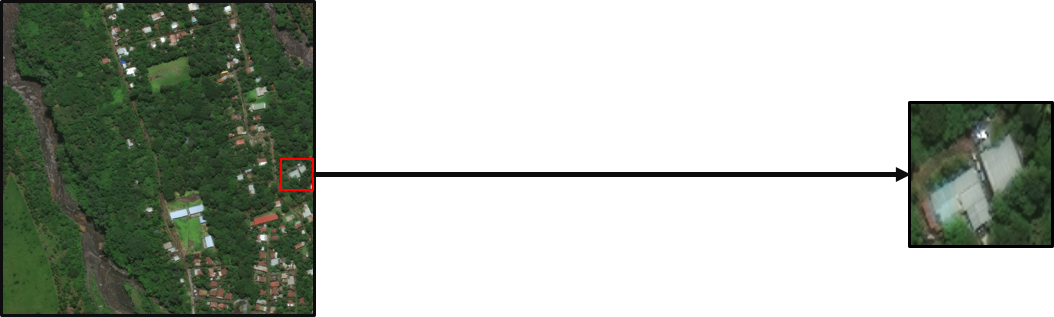
\includegraphics[width=\columnwidth , frame]{Image/Picture1.png}
    \caption{Data Prepossessing: Creating building patch  }
    \label{fig:outpur}
\end{figure}

\begin{figure*}[!t] % The asterisk makes it span two columns
    \centering
    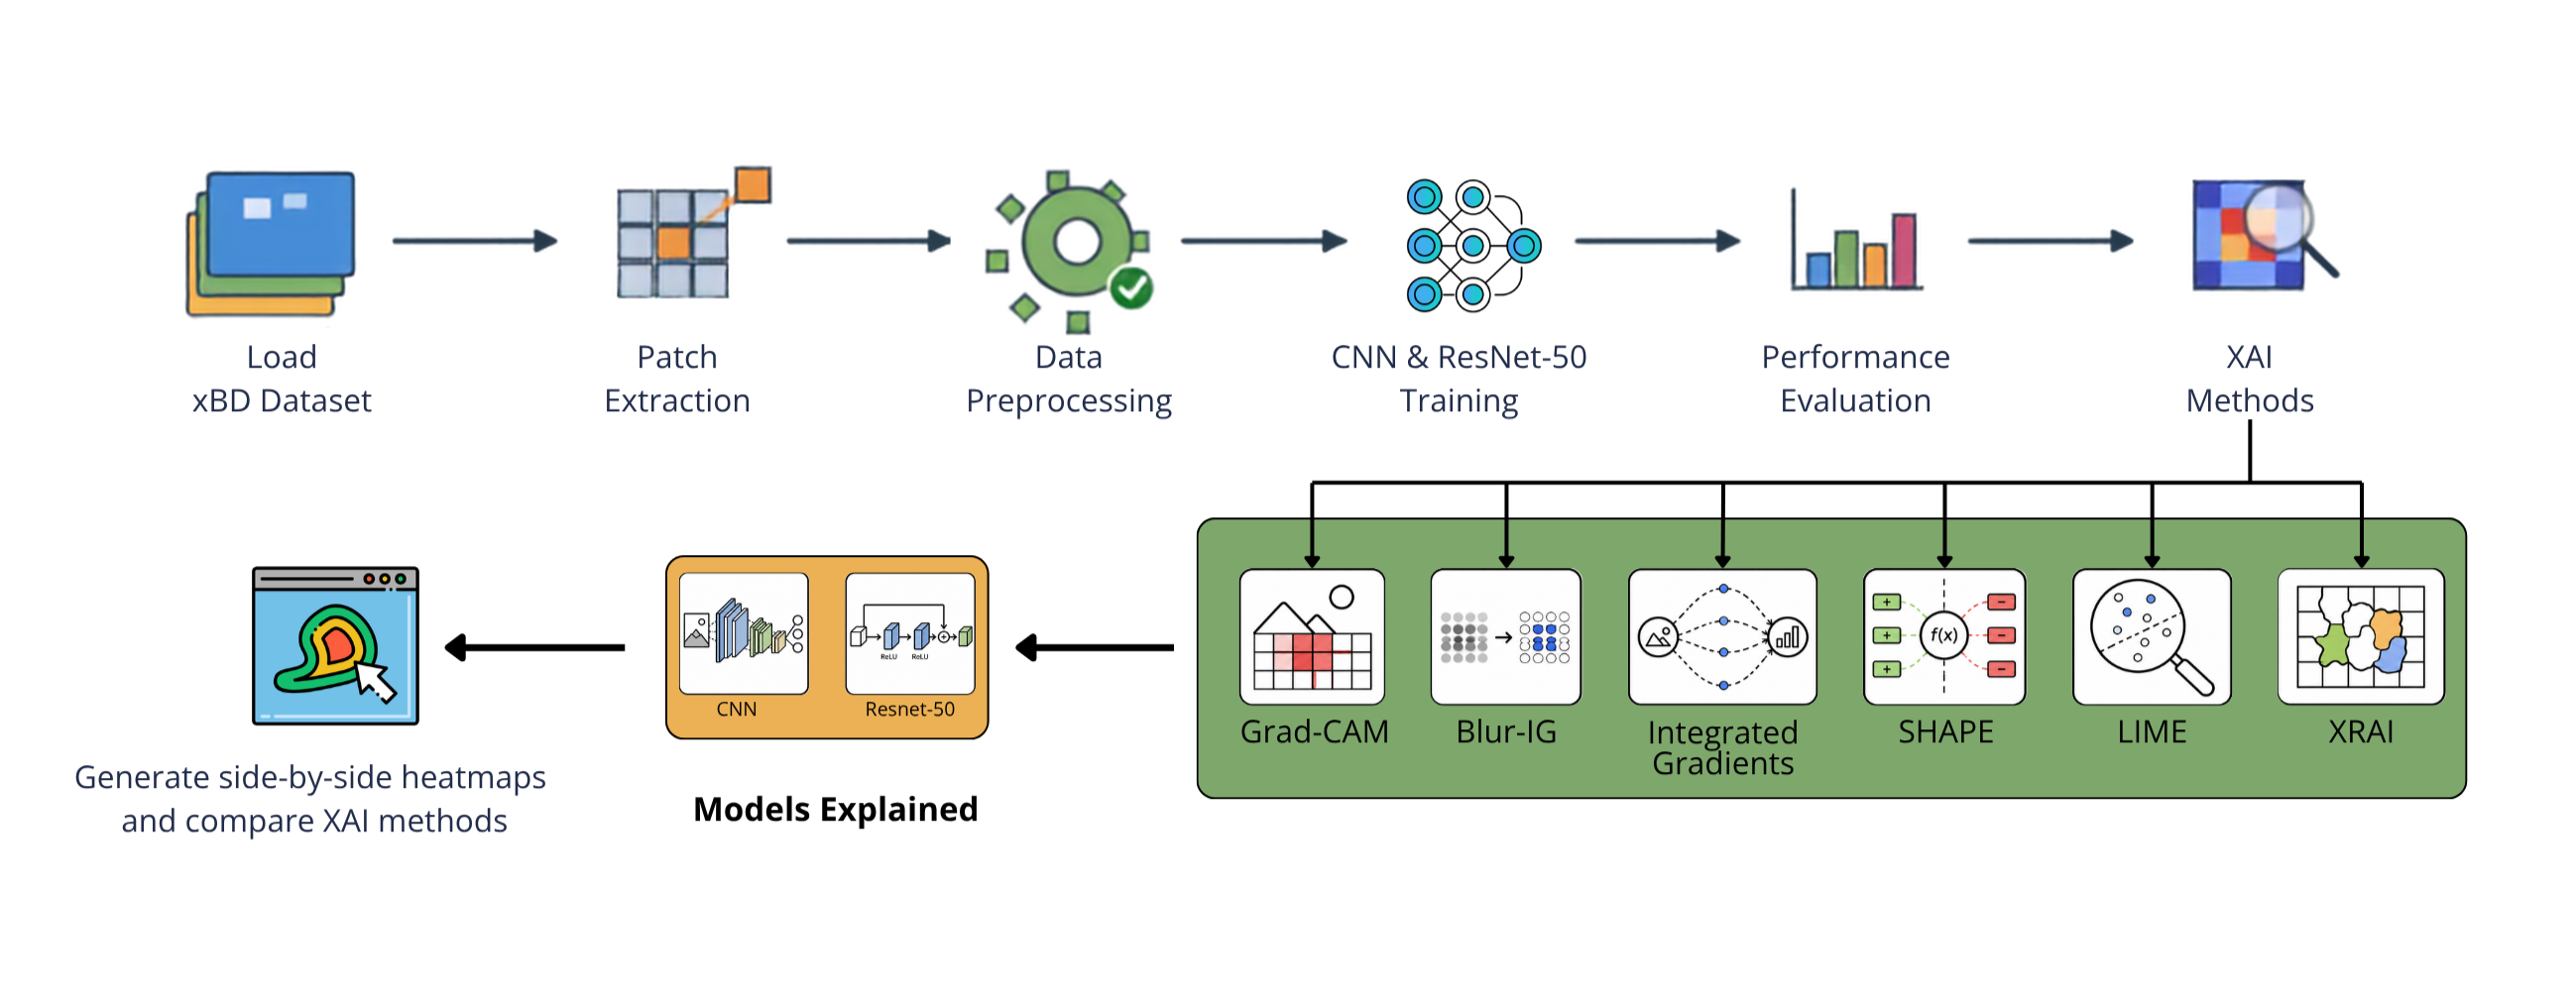
\includegraphics[width=\textwidth]{Image/Region-Based.png} 
    \caption{Framework for Explainable Post Disaster Building Damage AssesSment from Satellite Image}
    \label{fig:framework}
\end{figure*}


\subsection{Model}
\subsubsection{CNN}
{A Convolutional Neural Network (CNN) is a deep learning architecture used for processing image data. CNNs automatically learn features from image data through convolutional layers, pooling operations, and fully connected layers, progressing from low-level features such as edges and textures to higher-level patterns and object structures. In this study, a CNN is used for classifying building damage into four categories: no-damage, minor-damage, major-damage, and destroyed. This model receives an image as a multidimensional array of pixel values and processes it through a sequence of convolutional layers that apply learnable filters to extract spatial patterns and increasingly complex structural features. The extracted feature representations are subsequently passed to classification layers, where the final layer produces four output values corresponding to the four damage classes. %A softmax function is used to convert these outputs into class probabilities, and the class with the highest probability is selected as the predicted damage category. During training, the model parameters are optimized using the selected loss function and optimizer over multiple epochs, while validation is performed after each epoch to monitor validation loss, accuracy, macro F1-score, and per-class performance. This implementation enables the CNN to automatically learn relevant visual representations of building damage directly from the input images without relying on manually engineered features.}
\subsubsection{ResNet-50}
{ResNet-50 was implemented as a deep convolutional neural network for the same four-class building damage classification task. ResNet-50 contains approximately 50 layers and uses residual blocks with shortcut connections, which support effective training of deep networks and learning of complex visual features. A pretrained ResNet-50 model was adapted by replacing its original classification layer with a four-class output layer and fine-tuned using the prepared building-damage dataset, allowing previously learned visual features to be adapted to structural damage characteristics. 
%During training, model parameters were updated through backpropagation, while validation was performed after each epoch using validation loss, accuracy, macro F1-score, and per-class F1-score to evaluate classification performance.}
\subsection{XAI Model}
To improve the interpretability of the building damage classification models, six explainable artificial intelligence (XAI) techniques were considered: SHAP, XRAI, Grad-CAM, LIME, Integrated Gradients (IG), and Blur Integrated Gradients (Blur-IG). These methods provide complementary explanations of the model predictions by identifying image regions that contribute to the classification decision.
\subsubsection{SHAP}
SHAP attributes the model prediction to different input features by estimating their contribution to the output. For image classification, the resulting attribution map indicates regions that positively or negatively influence the predicted damage category.
\paragraph{XRAI}
XRAI generates region-based explanations by evaluating the importance of image areas and ranking them according to their contribution to the prediction. This provides a spatially coherent explanation that can be useful for identifying visually meaningful damage patterns.
\paragraph{Grad-CAM}
Grad-CAM uses the gradients of a target class with respect to the feature maps of a convolutional layer to generate a class-specific localization map. The resulting heatmap highlights regions that have the greatest influence on the model's predicted damage category.
\paragraph{LIME}
LIME explains an individual prediction by perturbing different regions of the input image and observing the resulting changes in the model output. An interpretable local surrogate model is then used to identify the image regions most influential to the prediction.
\paragraph{Integrated Gradients (IG)}
Integrated Gradients attributes the prediction to individual input pixels by accumulating gradients along a path from a baseline input to the original image. This produces an attribution map indicating the relative contribution of different image regions to the model prediction.
\paragraph{Blur Integrated Gradients (Blur-IG)}
Blur Integrated Gradients extends the Integrated Gradients approach by using progressively blurred versions of the input image along the attribution path. This provides a visually smooth attribution map and evaluates how the model's prediction changes as image information is gradually introduced.



\begin{figure*}[!t]
    \centering

    % Row 1
    \begin{subfigure}[b]{0.45\textwidth}
        \centering
        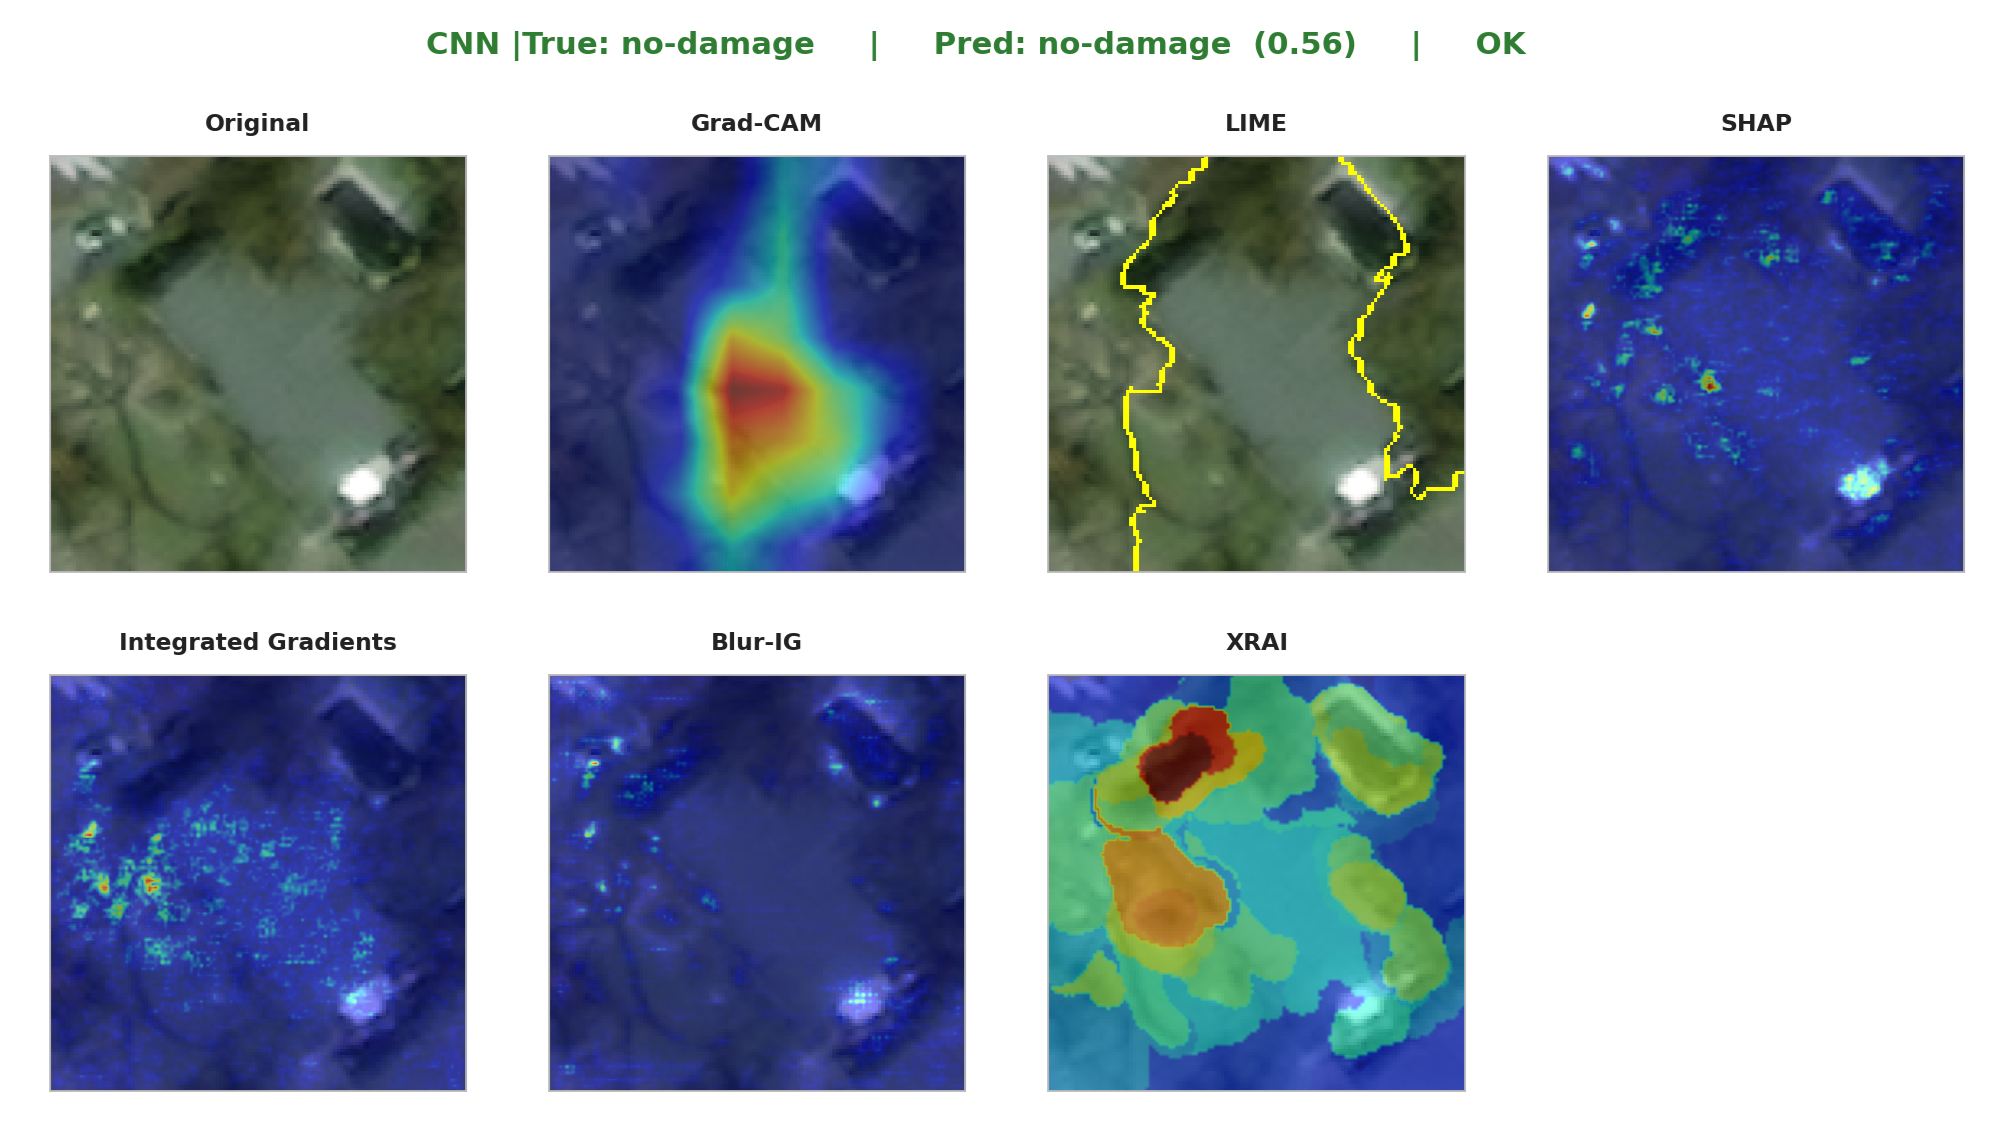
\includegraphics[width=\textwidth, frame]{Outputimg/cnn_08_OK_no-damage.png}
        \caption{CNN: No Damage}
        \label{fig:cnn_no_damage}
    \end{subfigure}
    \hfill
    \begin{subfigure}[b]{0.45\textwidth}
        \centering
        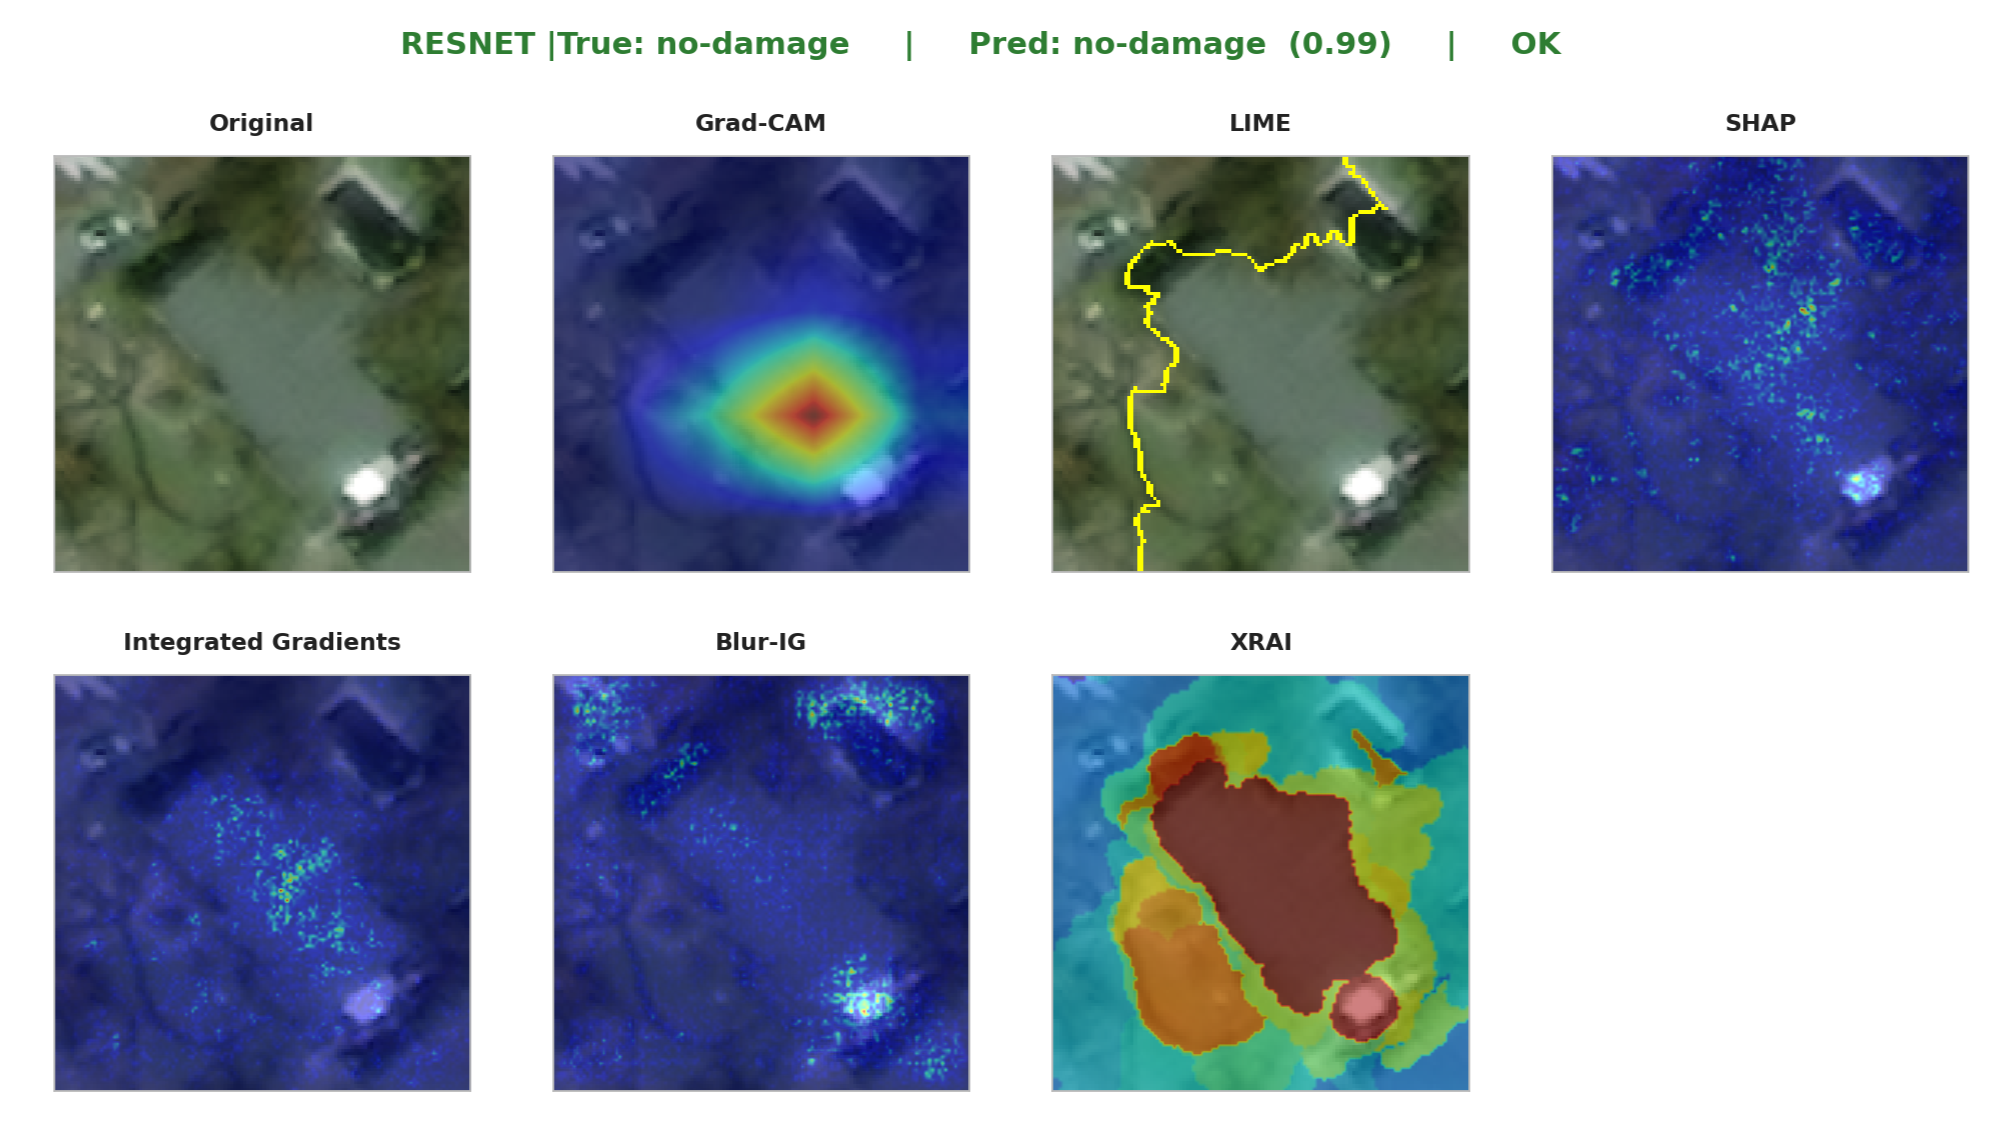
\includegraphics[width=\textwidth, frame]{Outputimg/resnet_08_OK_no-damage.png}
        \caption{ResNet-50: No Damage}
        \label{fig:resnet_no_damage}
    \end{subfigure}

    \vspace{0.1cm}

    % Row 2
    \begin{subfigure}[b]{0.45\textwidth}
        \centering
        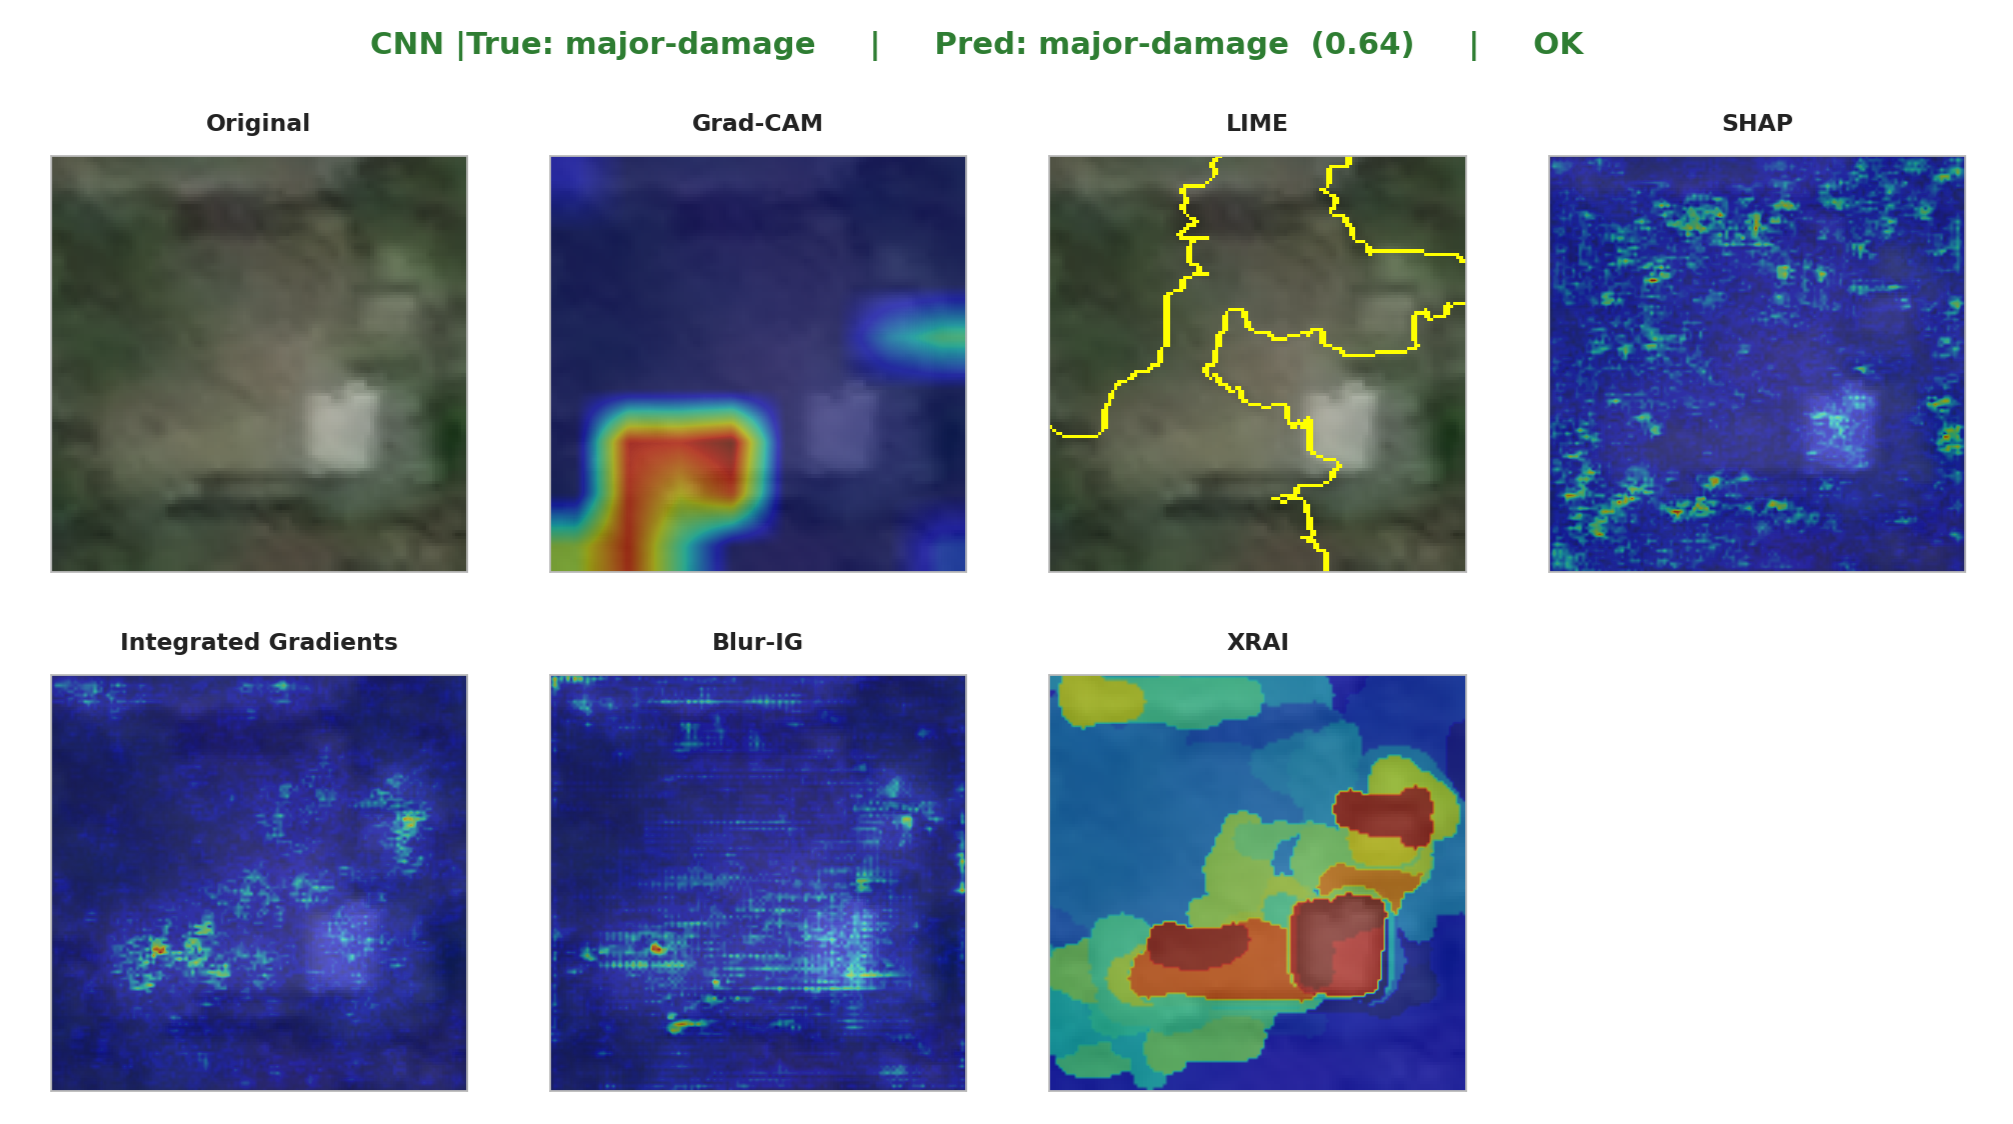
\includegraphics[width=\textwidth, frame]{Outputimg/cnn_14_OK_major-damage.png}
        \caption{CNN: Major Damage}
        \label{fig:cnn_major}
    \end{subfigure}
    \hfill
    \begin{subfigure}[b]{0.45\textwidth}
        \centering
        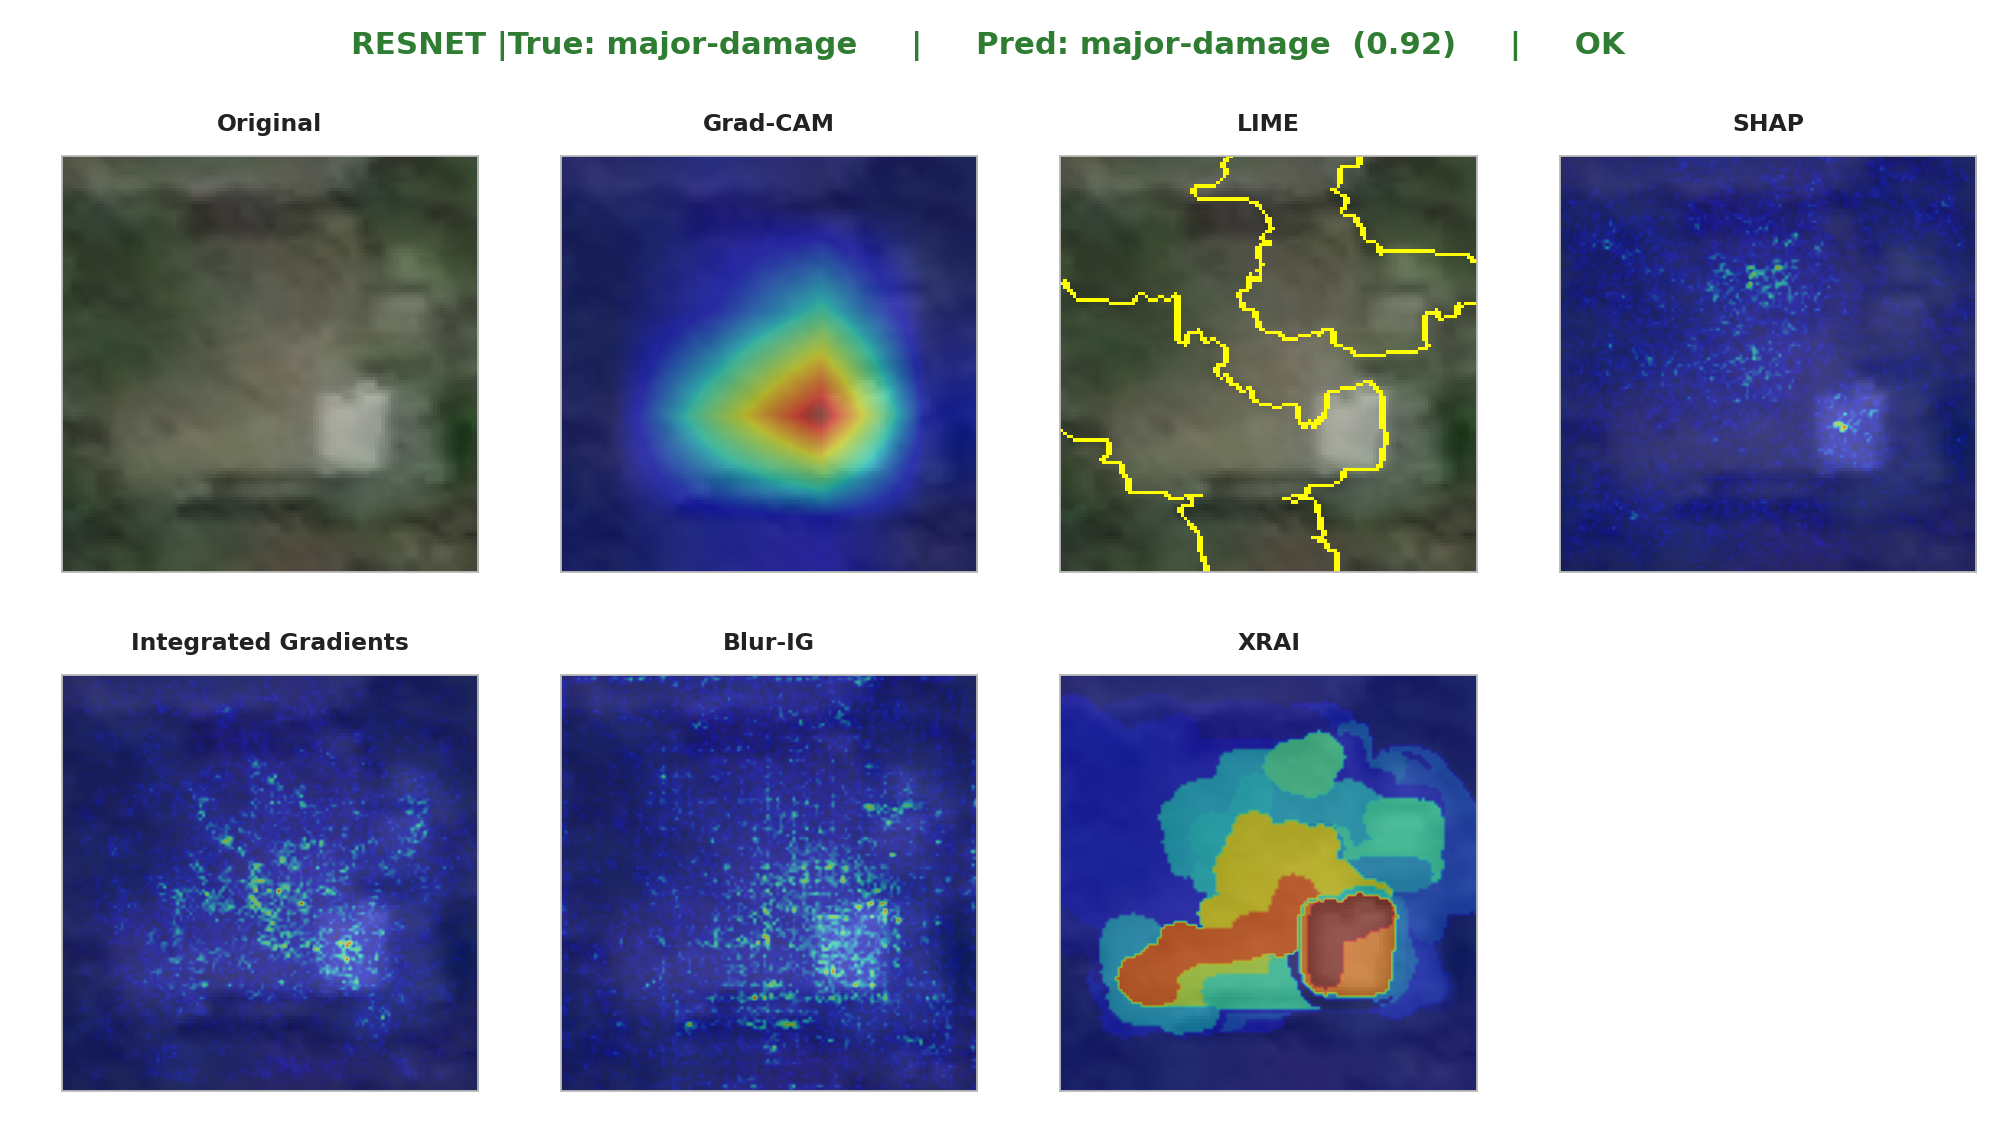
\includegraphics[width=\textwidth, frame]{Outputimg/resnet_14_OK_major-damage.png}
        \caption{ResNet-50: Major Damage}
        \label{fig:resnet_major}
    \end{subfigure}

    \vspace{0.1cm}

    % Row 3
    \begin{subfigure}[b]{0.45\textwidth}
        \centering
        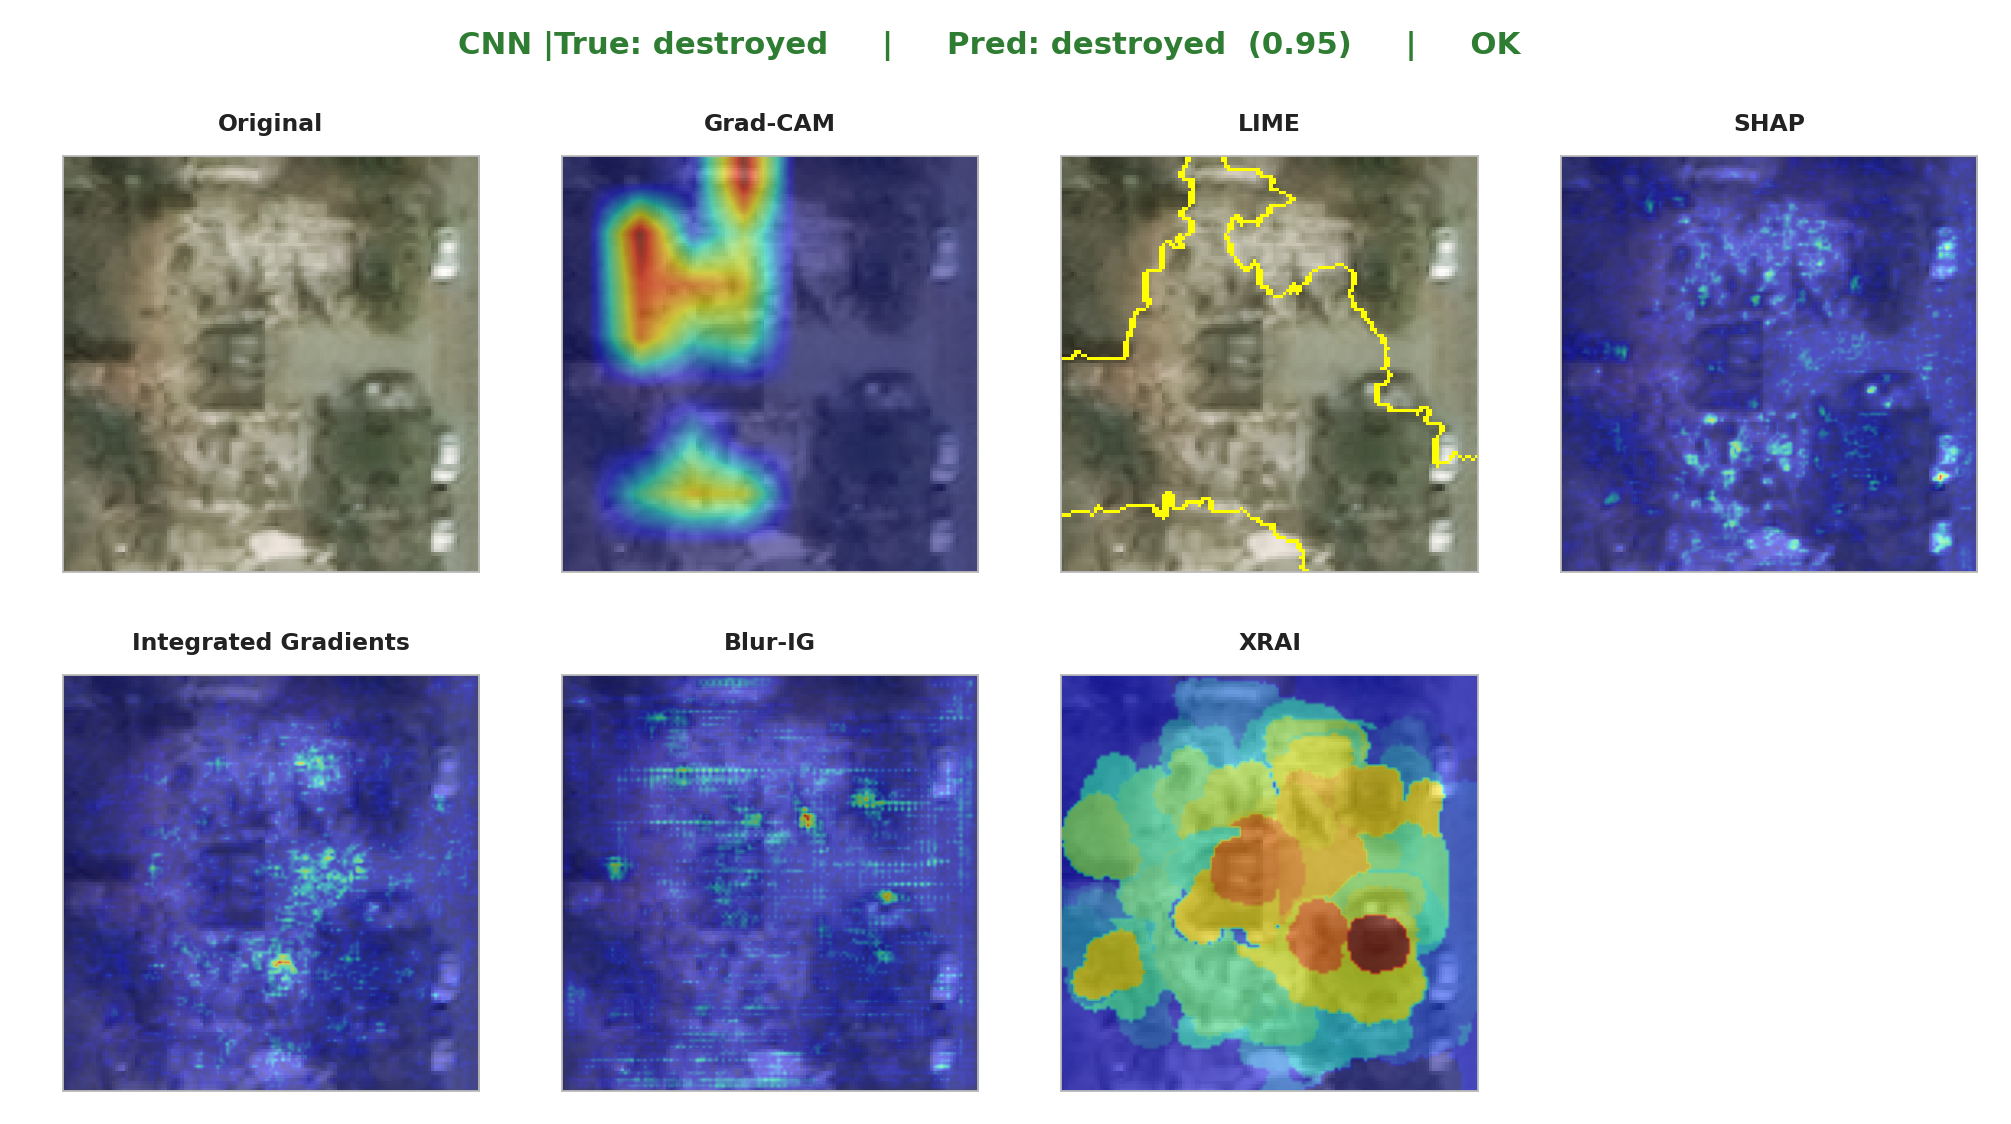
\includegraphics[width=\textwidth, frame]{Outputimg/cnn_06_OK_destroyed.png}
        \caption{CNN: Destroyed}
        \label{fig:cnn_destroyed}
    \end{subfigure}
    \hfill
    \begin{subfigure}[b]{0.45\textwidth}
        \centering
        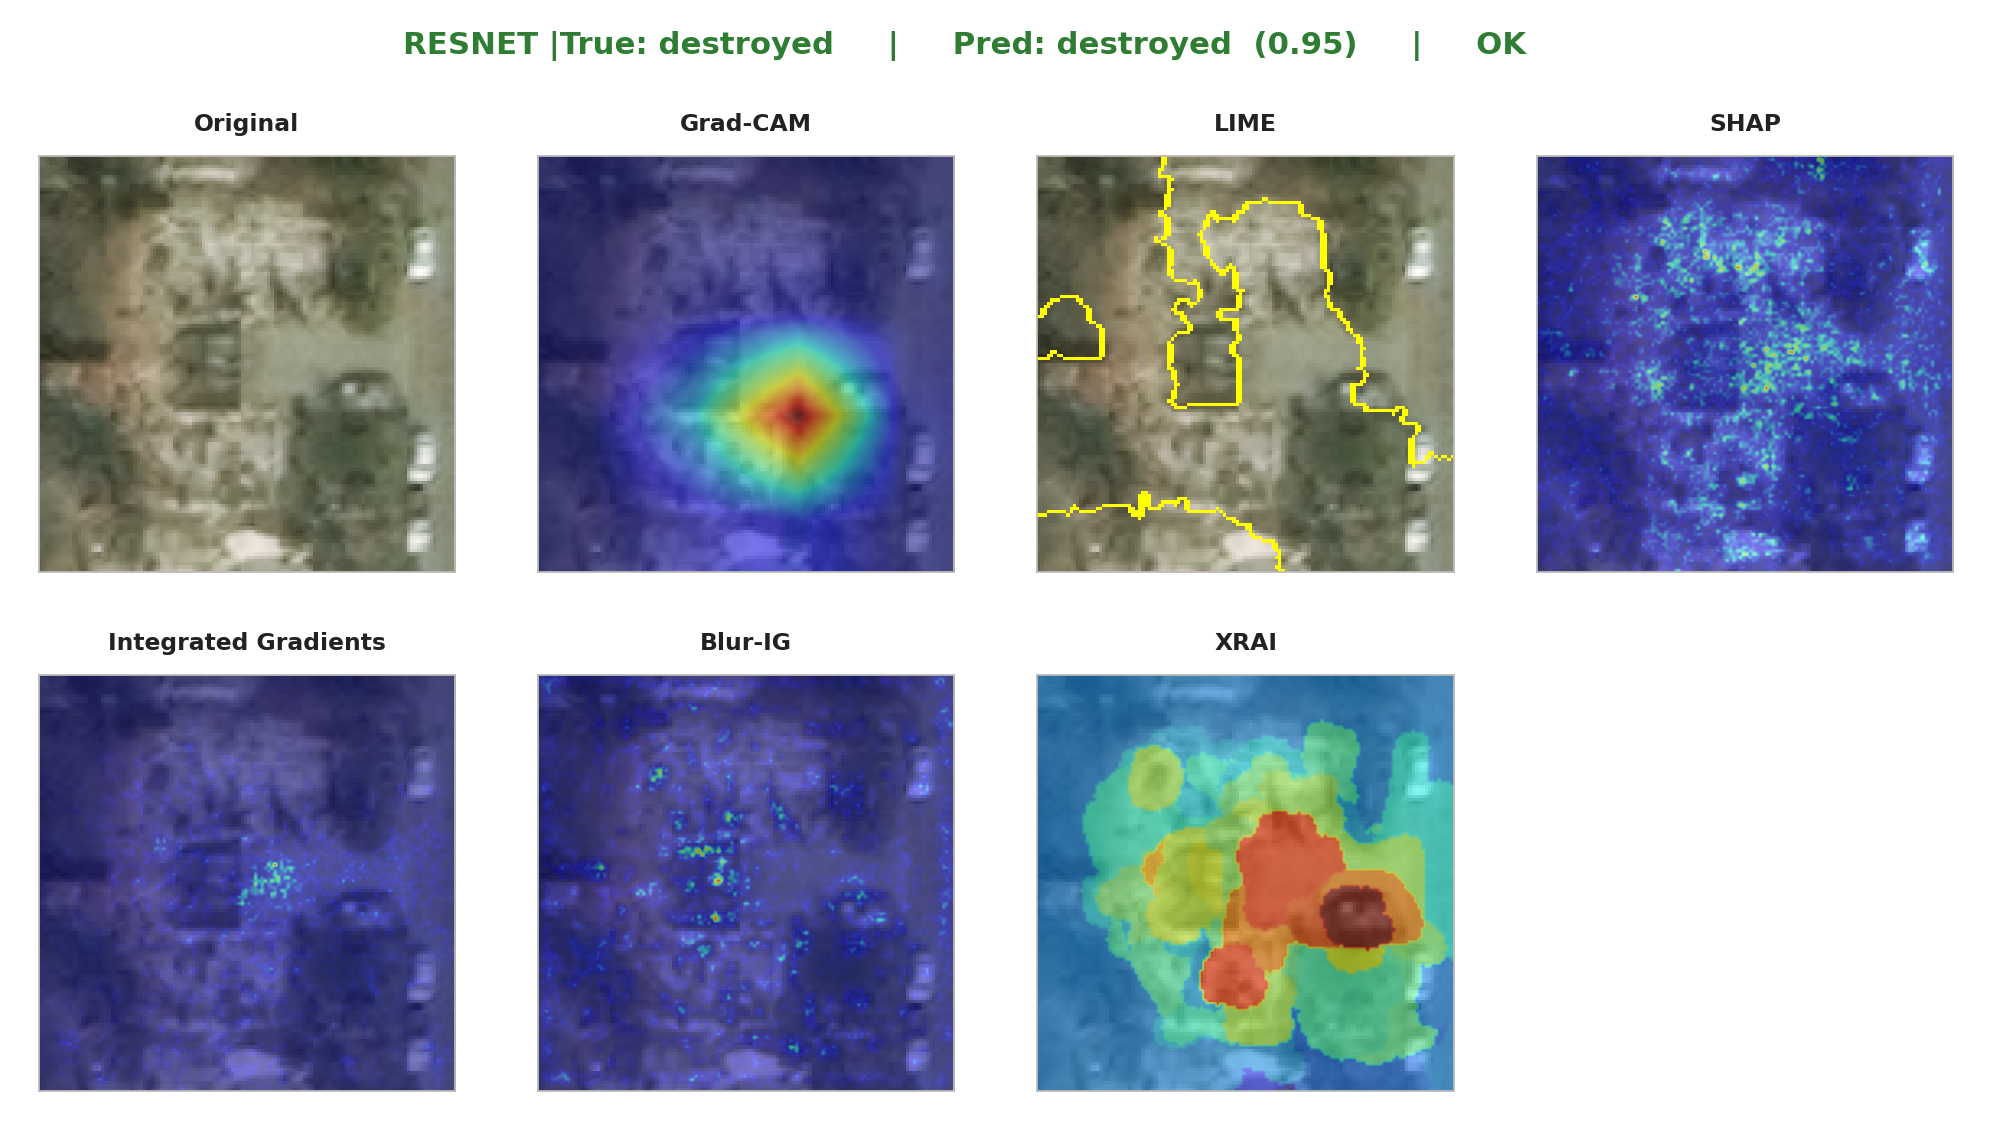
\includegraphics[width=\textwidth, frame]{Outputimg/resnet_06_OK_destroyed.png}
        \caption{ResNet-50: Destroyed}
        \label{fig:resnet_destroyed}
    \end{subfigure}
    
    \vspace{0.1cm}


    %row 4
    \begin{subfigure}[b]{.45\textwidth}
        \centering
        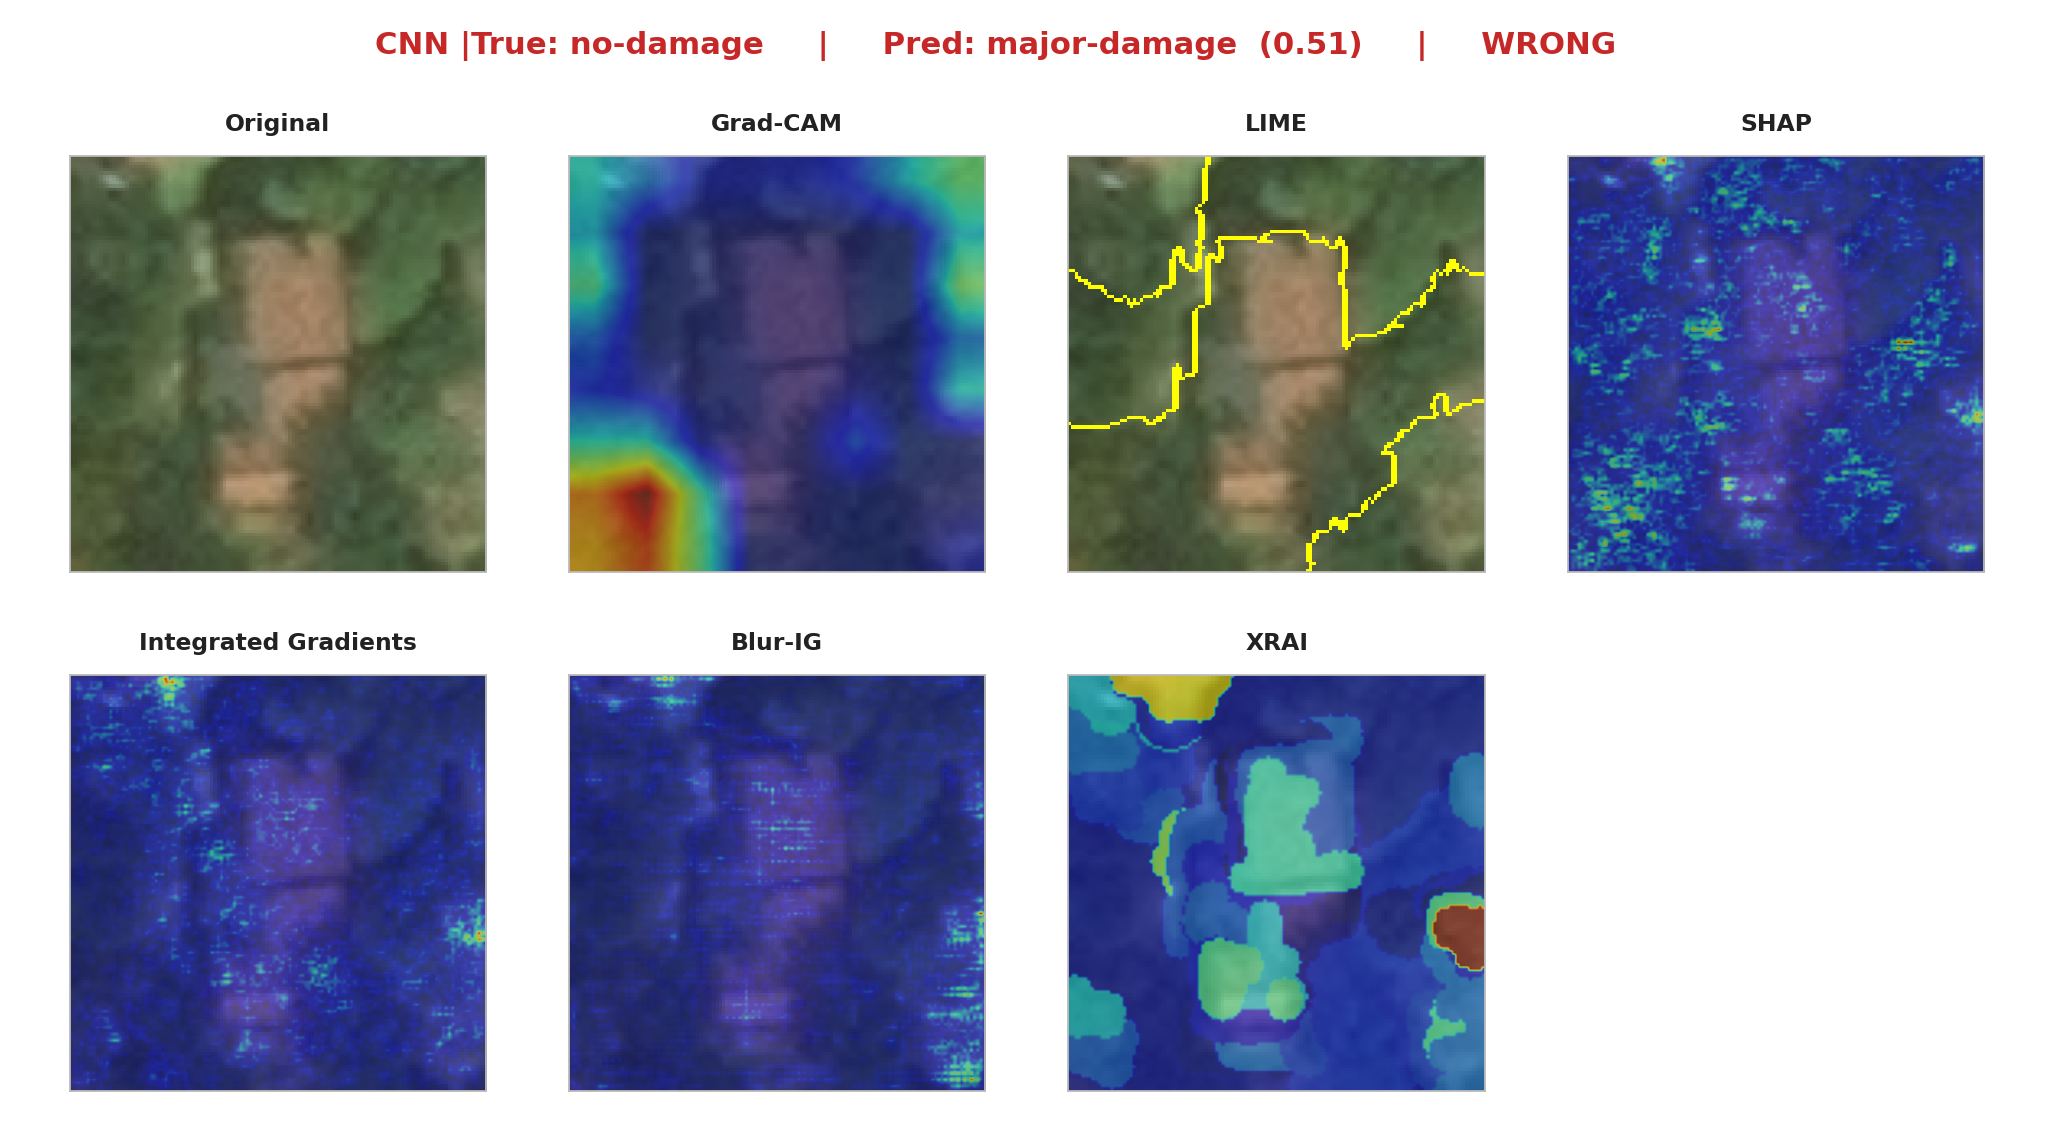
\includegraphics[width=\textwidth, frame]{Outputimg/cnn_04_WRONG_no-damage.png}
        \caption{CNN: Wrong Prediction}
        \label{fig:cnn_wrong}
    \end{subfigure}
    \hfill
    \begin{subfigure}[b]{.45\textwidth}
        \centering
        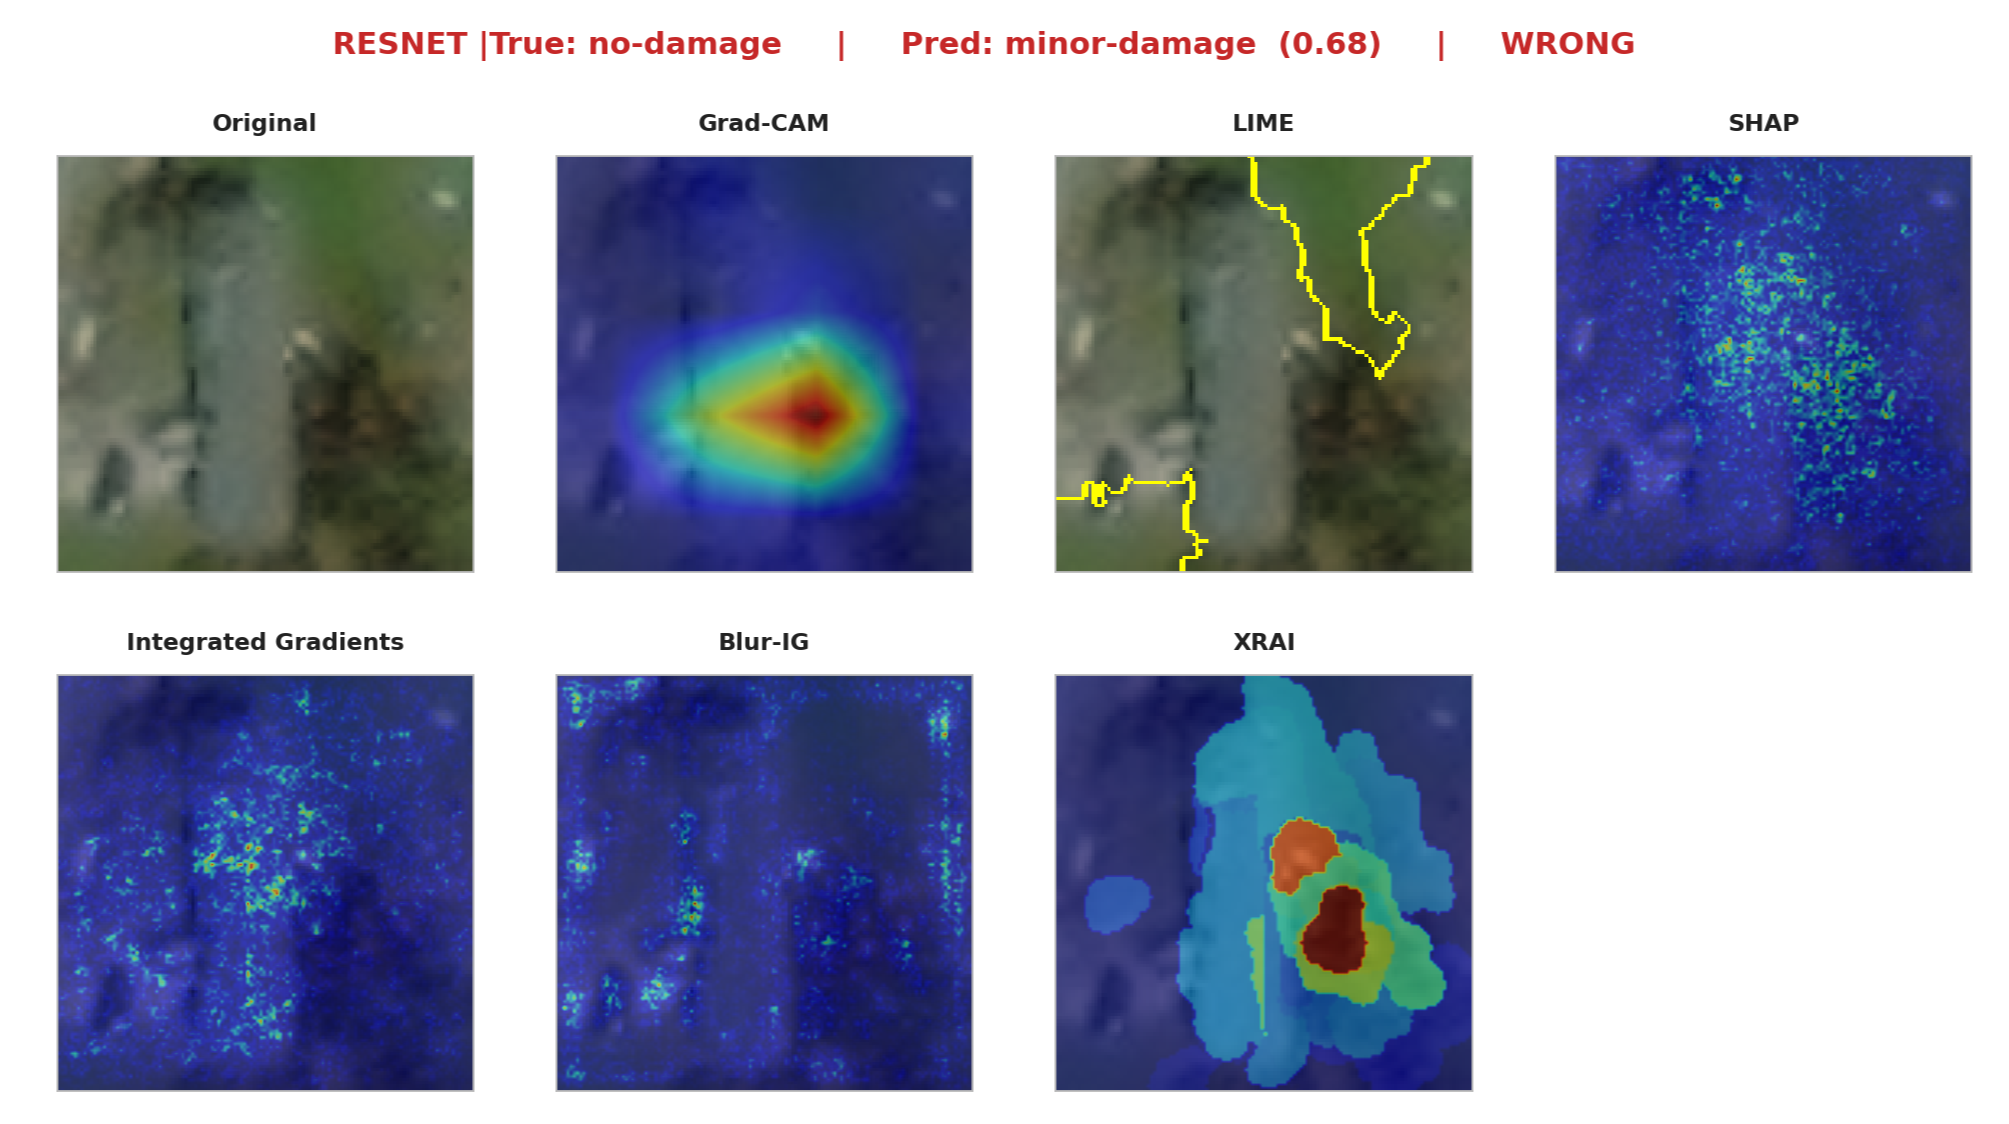
\includegraphics[width=\textwidth, frame]{Outputimg/resnet_04_WRONG_no-damage.png}
        \caption{ResNet-50: Wrong Prediction}
        \label{fig:resnet_wrong}
    \end{subfigure}
    

    \caption{Comparison of damage assessment predictions using CNN and ResNet-50.}
    \label{fig:damage_comparison}
\end{figure*}








\subsection{Proposed Framework}



Fig.~\ref{fig:framework} illustrates the overall framework of the architecture.





\subsection{Implementation}
\begin{algorithm}[H]
\caption{Model Architecture, Training, and Explainability Generation}
\label{alg:full}
\begin{algorithmic}[1]
\REQUIRE Train/Val/Test patches, Model type $\in$ \{CNN, ResNet-50\}
\ENSURE Trained model, XAI heatmaps

\IF{Model type = CNN}
    \STATE $h \leftarrow$ input patch $x \in \mathbb{R}^{128\times128\times3}$
    \FOR{each of 5 convolutional blocks}
        \STATE $h \leftarrow \text{MaxPool}(\text{ReLU}(\text{BatchNorm}(\text{Conv2D}(h))))$
    \ENDFOR
    \STATE $h \leftarrow \text{GlobalAvgPool}(h)$
    \STATE $\hat{y} \leftarrow \text{Softmax}(\text{FC}(\text{Dropout}(\text{FC}(h))))$
\ELSE
    \STATE Load ResNet-50 pretrained on ImageNet
    \STATE Freeze early layers (conv1, layer1, layer2)
    \STATE Replace final layer: Dropout $\rightarrow$ FC(4 classes)
    \STATE $\hat{y} \leftarrow \text{Softmax}(\text{ResNet-50 backbone}(x))$
\ENDIF
\STATE Apply weighted sampling for class balance
\FOR{each epoch}
    \FOR{each batch in Train set}
        \STATE Forward pass $\rightarrow$ compute cross-entropy loss
        \STATE Backpropagate and update weights
    \ENDFOR
    \STATE Evaluate on Val set $\rightarrow$ compute macro F1
    \IF{macro F1 improves}
        \STATE Save model checkpoint
    \ENDIF
\ENDFOR
\STATE Load best checkpoint $\rightarrow$ evaluate on Test set

\FOR{each test patch}
    \STATE Predict damage class using trained model
    \STATE Apply XAI methods (Grad-CAM, LIME, SHAP, IG, Blur-IG, XRAI)
    \STATE Generate side-by-side heatmap visualization
\ENDFOR

\end{algorithmic}
\end{algorithm}




\section{Results}


\subsection{Experimental Setup}
The xBD dataset splits: tier1, tier3 and train were used as training and validation sets. The test and hold split were not used during model train as they were reserved as an independent test set for final evaluation. Buildings were extracted from the post-disaster images. 300,000 samples were for training and validation , 106787 samples for independent test set distributed across four category: no-damage, minor-damage, major-damage, and destroyed.To prevent data leakages data splits were constructed scens-wise by disaster event.
Two architecture were trained under identical conditions. A CNN trained from the scratch (1.7M parameters) and a ResNet-50 pretrained on ImageNet and fine-tuned via transfer learning(23M parameters). In both model used AdamW optimizer, cosine annealing learning rate schedule and cross entropu loss with labeling smoothing. The CNN was trained for 25 epochs but the best epoch is 21, batch size 128 and learning rate $1 \times 10^{-4}$. The Resnet-50 was trained for 15 epochs and it was the the best epoch. Batch size was 96 and learning rate was $1 \times 10^{-4}$. Best Model selection was based on validation macro F1-score. It was alos evaluated on the independent test set.
%For explainability, six methods across three families were applied to both models. From gradient-based: Grand-cam, Integrated Gradients, Blur-IG, From perturbation-base: LIME, SHAP, and from region based: XRAI was used. All generated for both correct and incorrect classified test samples. 
\subsection{Model Evaluation}

 In Table~\ref{tab:cnn_resnet_comparison} a performance comparison is given between our train model: CNN and ResNet-50. From this table it is observed that ResNet-50 perform better than CNN with  84.12\% accuracy and 84.98\% F1-score. While CNN has 79.62\% accuracy and 81.80\% F1-score. The results show that ResNet-50 provides better  performance for building damage classification.

% ---------------- Table ----------------
 
\begin{table}[h]
\centering
\caption{Performance Comparison between CNN and ResNet Models}
\label{tab:cnn_resnet_comparison}
\resizebox{\columnwidth}{!}{%
\begin{tabular}{lccccc}
\hline
\textbf{Model} & \textbf{Best Epoch} & \textbf{Accuracy (\%)} &
\textbf{Precision (\%)} & \textbf{Recall (\%)} & \textbf{F1-Score (\%)} \\
\hline
CNN    & 21 & 79.62 & 86.22 & 79.62 & 81.80 \\
ResNet & 15 & \textbf{84.12} & \textbf{86.25} & \textbf{84.12} & \textbf{84.98} \\
\hline
\end{tabular}%
}
\end{table}

\subsection{XAI Result}

In figure \ref{fig:cnn_no_damage} we can see the building is classified as no-damage category by CNN Model. The heatmap generated by the XAI tools also over the building. The same image is also classified as no damage by ResNet-50. In figure \ref{fig:resnet_no_damage} we can see the heatmap generated by XAI tool is also over the building. Similarly in figure \ref{fig:cnn_major}
and figure \ref{fig:resnet_major} we can see both model classified the building as major-damage. But the heatmap generated by XAI Tools highlight different part of building in this two model. Same result we can also observe in figure \ref{fig:cnn_destroyed} and figure \ref{fig:resnet_destroyed}.  In figure \ref{fig:cnn_wrong} we can see the building is classified as major damage but the XAI tools show the heatmap is not over the building. So this result by CNN model is wrong as it did not take decision from the building. Similarly in figure \ref{fig:resnet_destroyed} we can see ResNet-50 classified the building as minor-damage. But XAI tools did not generate the heatmap over the building. So, from XAI it is clear that the result is not correct. 
\subsection{Comparison of XAI}
Comparison of XAI is difficult as it's effectiveness depends on the human inspection. But to identify which XAI better three methods are followed. They are Intersection Over Union(IoU), Faithfulness, and computational runtime.  Figure \ref{fig:xai-comp} shows the how the IoU measure.  Figure \ref{fig:xai-faith} shows the process of measurement of faithfulness.
\begin{figure}[h] % The asterisk makes it span two columns
    \centering
    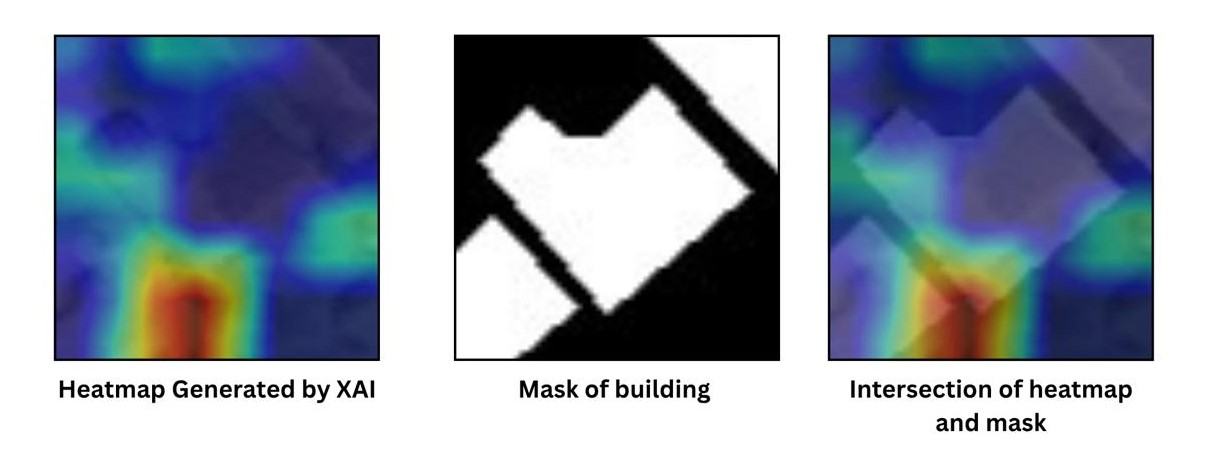
\includegraphics[width=\columnwidth]{Image/WhatsApp Image 2026-08-20 at 9.41.15 AM.jpeg} 
    \caption{ Process of Measuring Interaction over Union }
    \label{fig:xai-comp}
\end{figure} 
 
\begin{figure}[h] % The asterisk makes it span two columns
    \centering
    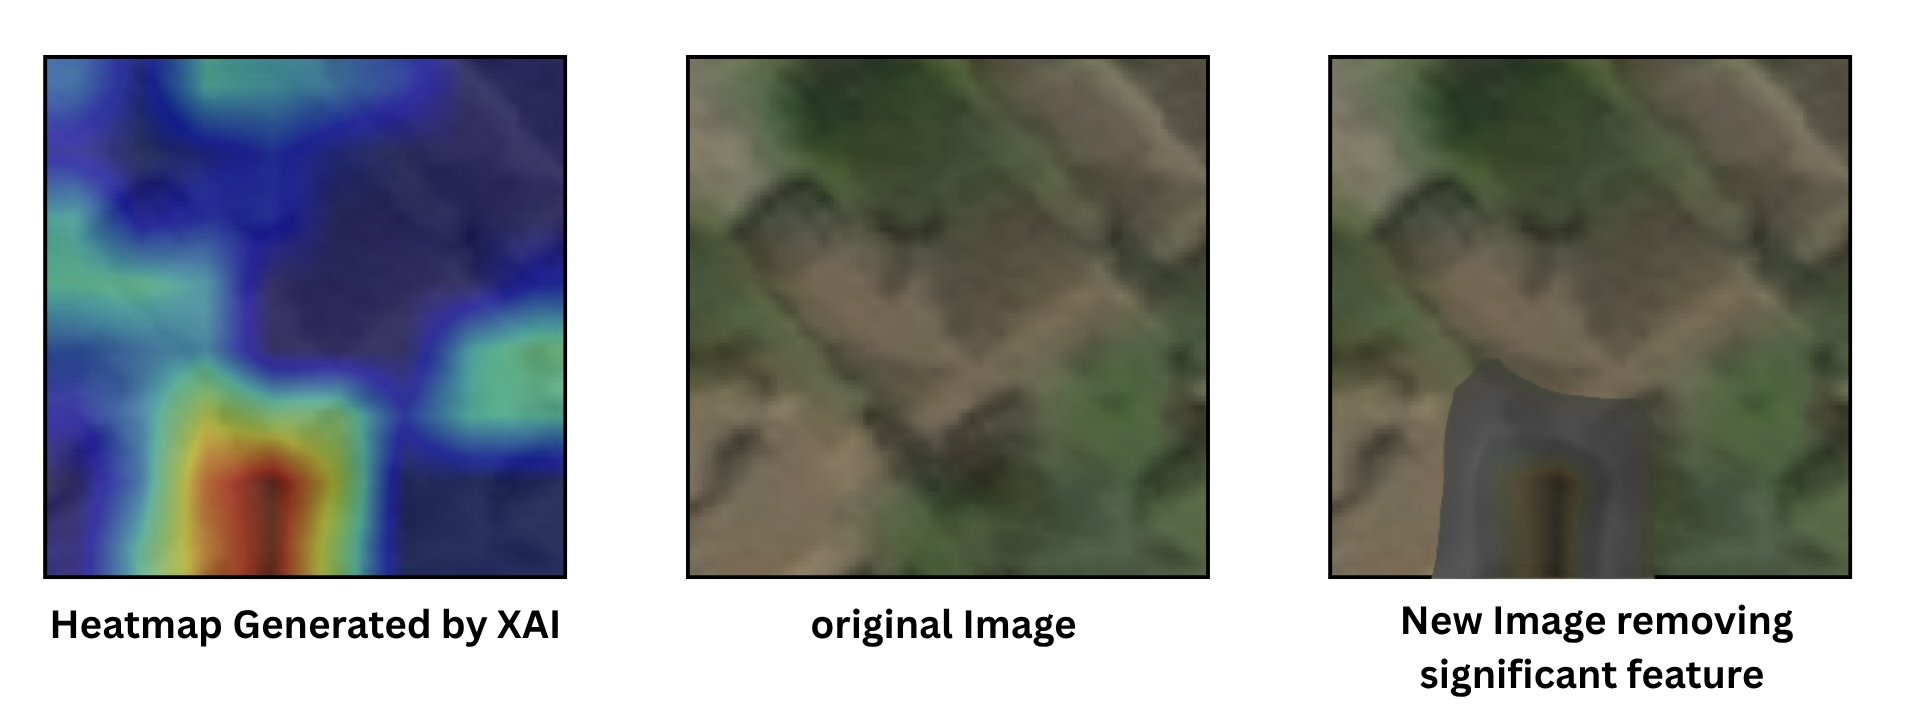
\includegraphics[width=\columnwidthwidth ]{Image/Add a subheading.jpeg} 
    \caption{ Process of Measuring Faithfulness }
    \label{fig:xai-faith}
\end{figure}

 400 samples , 100 sample from each category is taken. From this samples set the mean value was taken. Table \ref{tab:xai_cnn_resnet} shows the mean value of IoU, Faithfulness, and computational runtime of each XAI.

\begin{table}[htbp]
\centering
\caption{Comparison of XAI Models on CNN and ResNet-50}
\label{tab:xai_cnn_resnet}
\resizebox{\columnwidth}{!}{%
\begin{tabular}{lcccccc}
\toprule
\textbf{XAI Model} 
& \multicolumn{3}{c}{\textbf{CNN}} 
& \multicolumn{3}{c}{\textbf{ResNet-50}} \\
\cmidrule(lr){2-4}
\cmidrule(lr){5-7}
& \textbf{IoU} & \textbf{Faith.} & \textbf{Runtime}
& \textbf{IoU} & \textbf{Faith.} & \textbf{Runtime} \\
\midrule
Grad-CAM
& 0.1560 & 0.2886 & 0.0050
& 0.3886 & 0.2936 & 0.0178 \\

LIME
& 0.2172 & 0.2390 & 0.8240
& 0.2004 & 0.2747 & 1.1957 \\

SHAP
& 0.1668 & 0.3458 & 1.3116
& 0.2079 & 0.6075 & 2.6410 \\

Integrated Gradients
& 0.1973 & 0.3150 & 0.0742
& 0.2321 & 0.5935 & 0.3221 \\

Blur-IG
& 0.1454 & 0.3214 & 1.0770
& 0.1493 & 0.5845 & 1.5523 \\

XRAI
& 0.2189 & 0.2481 & 1.5558
& 0.3385 & 0.3204 & 4.0080 \\

\bottomrule
\end{tabular}%
}
\end{table}


From the table, Grad-CAM was faster in both CNN and Resnet-50. On the other hand, XRAI was slower in both models. But in CNN model  XRAI had max IoU. In ResNet-50 model, Grand-CAM had maximum IoU value. In term of faithfulness, SHAP had max value in both model. If we consider the balance performance then Integrated Gradients can be consider better. A noticable pattern is that all the XAI perform better in the ResNet-50 model. 

\section{Conclusion}
This study includes a building-level damage classification methodology that used the xBD dataset, comparing the performance of a simple CNN and ImageNet-pretrained ResNet-50 classifiers using 4 categories. The scene-wise data split and imbalance-aware sampling strategies reduced data leakage and bias, while the application of six XAI methods, namely, SHAP, XRAI, Grad-CAM, LIME, Integrated Gradients, and Blur Integrated Gradients, enhanced the interpretability of results. The ResNet-50 model achieved the better performance, yet the CNN classifier showed comparable accuracy with a much lower number of parameters.

%Future research should focus on improving the recognition of buildings with minor and major damage, which proved to be more challenging than distinguishing between no damage and destroyed buildings. Other avenues of future research include exploring alternative architectures and considering models pretrained on satellite-specific data, applying the current approach to new disasters and localities, and conducting quantitative comparisons of the consistency and reliability of different XAI methods.

% ---------------- References ----------------
% Option 1: manual bibliography (simplest, used below)
\begin{thebibliography}{00}
\bibitem{wang2026bda} Y. Wang, J. Cui, C. Zhai, X. Tao, and Y. Li, ``Integrating segmentation and vision-language model for automated and interpretable building damage assessment from satellite imagery,'' \textit{Adv. Eng. Inform.}, vol. 71, p. 104320, 2026.

\bibitem{lagap2025xai} U. Lagap, S. Ghaffarian, S. Gelinas-Gagne, J. Jilma, Z. Liu, and Z. Luo, ``Towards reliable deep learning for post-disaster damage assessment: An XAI-based evaluation,'' \textit{Int. J. Disaster Risk Reduction}, vol. 130, p. 105839, 2025.

\bibitem{gu2025seismic} Y. Gu, S. Yang, X. Zhou, and Y. Liu, ``Explainable seismic damage prediction model based on CELS-WOA-stacking,'' \textit{Adv. Eng. Inform.}, vol. 66, p. 103430, 2025.

\bibitem{multiscale2026} ``A multi-scale deep learning framework for real-time post-earthquake damage estimation leveraging wavelet-driven GoogLeNet-FC,'' \textit{Soil Dyn. Earthquake Eng.}, vol. 204, p. 110084, 2026.

\bibitem{khorram2021xai} S. Khorram \textit{et al.}, ``Earthquake-induced building-damage mapping using explainable AI (XAI),'' \textit{Sensors}, vol. 21, no. 13, p. 4489, 2021.
\bibitem{gupta2019xbd} R. Gupta \textit{et al.}, ``Creating xBD: A dataset for assessing building damage from satellite imagery,'' in \textit{Proc. IEEE/CVF Conf. Comput. Vis. Pattern Recognit. Workshops}, 2019, pp. 10--17.

\bibitem{selvaraju2017gradcam} R. R. Selvaraju, M. Cogswell, A. Das, R. Vedantam, D. Parikh, and D. Batra, ``Grad-CAM: Visual explanations from deep networks via gradient-based localization,'' in \textit{Proc. IEEE Int. Conf. Comput. Vis.}, 2017, pp. 618--626.

\bibitem{lundberg2017shap} S. M. Lundberg and S.-I. Lee, ``A unified approach to interpreting model predictions,'' in \textit{Adv. Neural Inf. Process. Syst.}, vol. 30, 2017, pp. 4765--4774.

\bibitem{ribeiro2016lime} M. T. Ribeiro, S. Singh, and C. Guestrin, ````Why should I trust you?'': Explaining the predictions of any classifier,'' in \textit{Proc. 22nd ACM SIGKDD Int. Conf. Knowl. Discovery Data Mining}, 2016, pp. 1135--1144.

\bibitem{ma2024transfer} Y. Ma, S. Chen, S. Ermon, and D. B. Lobell, ``Transfer learning in environmental remote sensing,'' \textit{Remote Sens. Environ.}, vol. 301, p. 113924, 2024.

\bibitem{plested2026transfer} J. Plested, M. Phiri, and T. Gedeon, ``Deep transfer learning for image classification: A survey,'' \textit{Artif. Intell. Rev.}, vol. 59, no. 100, 2026.

\end{thebibliography}

% Option 2: BibTeX (uncomment these two lines, comment out the block
% above, and add a references.bib file to your project)
% \bibliographystyle{IEEEtran}
% \bibliography{references}

\end{document}
